\section{Iteration \#3 -- $kd$-Tree Exploration}

This iteration explores a widely used index structure based on spatial decomposition, instead of using dimension reduction via a hashing function. Different variations of this structure are implemented and evaluated alongside the best performing hash-based approaches from the previous iterations.

\subsection{Point $kd$-Tree}

The $kd$-Tree variant described in Section \ref{sec:kd-tree-chosen} was implemented, which shall be referred to as the \textbf{Point $kd$-Tree}. Each node is represented as a C-struct which stores a single point as well as pointers to its children. Every node is allocated using a call to \texttt{malloc()}, which allocates enough memory on the heap to store the node. This means each node may reside in different areas of the heap, resulting in fragmented memory.

\subsection{Bucket $kd$-Tree}

Instead of storing a single point in every node of the tree, the \textbf{Bucket $kd$-Tree} stores multiple points (i.e. a bucket) in nodes, with the constraint that only leaf nodes store points. Non-leaf nodes serve to partition the data space, each cutting the space along a single dimension by some value (the cutting value). When the number of points in a leaf exceeds a certain number, say $M$, then a cutting dimension and value are determined and the node is \textit{split} into two. The left and right children nodes are leaves that contain the points from the split node that lie on one of the sides of the cutting dimension. This process is illustrated in Figure \ref{fig:kd-split}.

To query or deleting a point, the leaf containing the point is found, which is sequentially scanned to find the point. After removing a point, the total number of points being stored in the modified leaf node and its sibling is less than $\frac{M}{4}$, then the two leaf nodes are \textit{merged} into their parent. The parent becomes a leaf node (see \ref{fig:kd-merge}) containing all the points from the two leaves.

With this approach, the tree has more knowledge about the distribution of the points to determine a more effective way partition the data which ensures the search tree is balanced. With the Point $kd$-Tree, only one point at a time is used to determine the cutting dimension. There is also less heap fragmentation because the points stored in leaves are stored contiguously.

TODO: two figures??

\subsection{Performance Timings}

TODO

\begin{table}
	\centering
	\makebox[\textwidth][c]{%
		\begin{tabular}{|r|r|l|l|l|l|l|l|l|l|}
			\hline
			\multicolumn{2}{|c}{} & \multicolumn{8}{|c|}{\textbf{Dimensionality}} \\
			\hline
			\textbf{Structure} & \textbf{Operation} & 1 & 2 & 3 & 5 & 10 & 50 & 100 & 200 \\
			\hline
			\multirow{3}{*}{Bucket PPT} & Insert & TODO & TODO & TODO & TODO & TODO & TODO & TODO & TODO \\
				& Delete & TODO & TODO & TODO & TODO & TODO & TODO & TODO & TODO \\
				& PQuery & TODO & TODO & TODO & TODO & TODO & TODO & TODO & TODO \\
			\hline			
			\multirow{3}{*}{Bucket PT} & Insert & TODO & TODO & TODO & TODO & TODO & TODO & TODO & TODO \\
				& Delete & TODO & TODO & TODO & TODO & TODO & TODO & TODO & TODO \\
				& PQuery & TODO & TODO & TODO & TODO & TODO & TODO & TODO & TODO \\
			\hline			
			\multirow{3}{*}{Bucket Hash Table} & Insert & TODO & TODO & TODO & TODO & TODO & TODO & TODO & TODO \\
				& Delete & TODO & TODO & TODO & TODO & TODO & TODO & TODO & TODO \\
				& PQuery & TODO & TODO & TODO & TODO & TODO & TODO & TODO & TODO \\
			\hline
			\multirow{3}{*}{Point $kd$-Tree} & Insert & TODO & TODO & TODO & TODO & TODO & TODO & TODO & TODO \\
				& Delete & TODO & TODO & TODO & TODO & TODO & TODO & TODO & TODO \\
				& PQuery & TODO & TODO & TODO & TODO & TODO & TODO & TODO & TODO \\
			\hline
			\multirow{3}{*}{Bucket $kd$-Tree} & Insert & TODO & TODO & TODO & TODO & TODO & TODO & TODO & TODO \\
				& Delete & TODO & TODO & TODO & TODO & TODO & TODO & TODO & TODO \\
				& PQuery & TODO & TODO & TODO & TODO & TODO & TODO & TODO & TODO \\
			\hline
		\end{tabular}
	}%

	\caption{Total Execution Time (in seconds) of Each Operation for Varying Number of Dimensions in Uniformly Distributed Synthetic Dataset}
	\label{tab:perf3-dimensionality}
\end{table}

\begin{figure}
	\begin{center}
		\begin{subfloat}[\texttt{insert}\label{fig:perf3-dimensionality-insert}]{%
			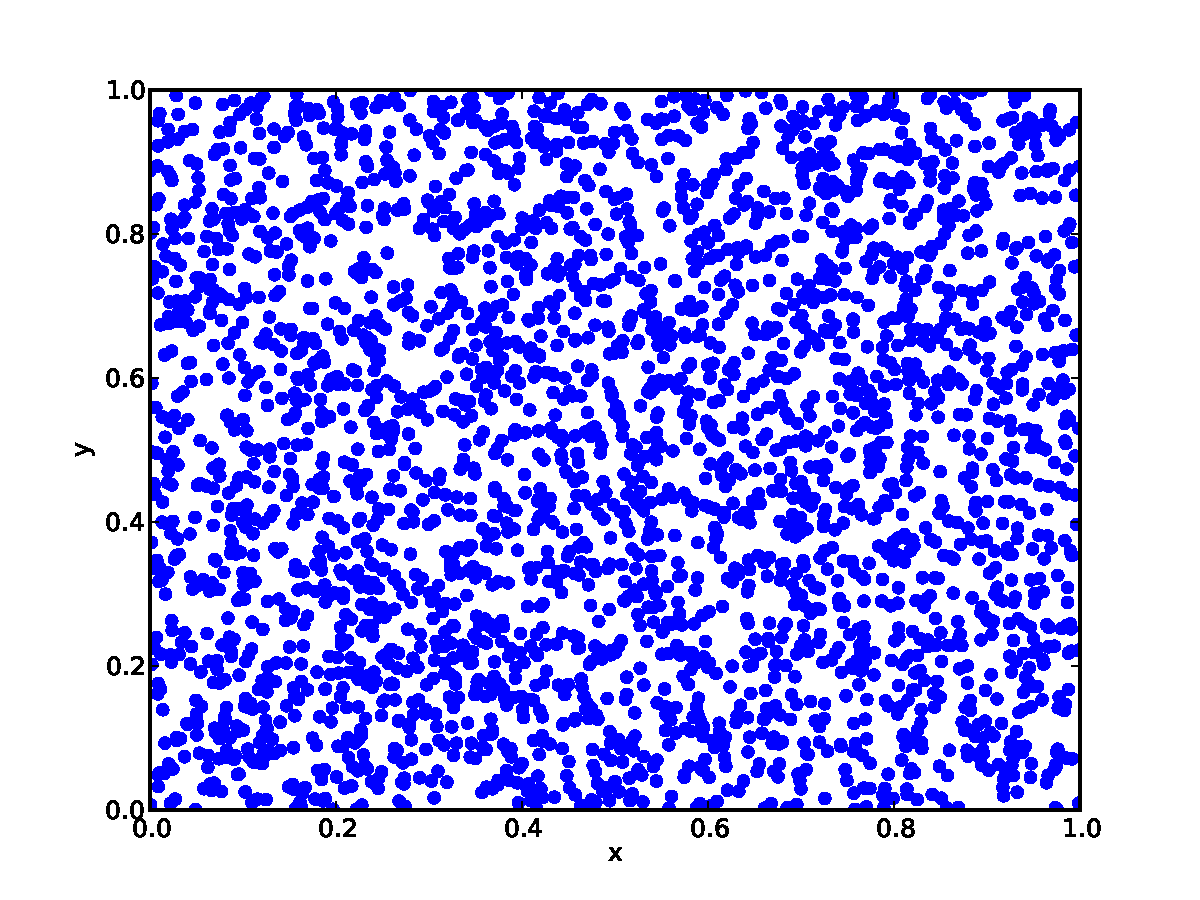
\includegraphics[scale=0.25]{figures/uniform_distribution.pdf}
		}
		\end{subfloat}~
		\begin{subfloat}[\texttt{remove}\label{fig:perf3-dimensionality-remove}]{%
			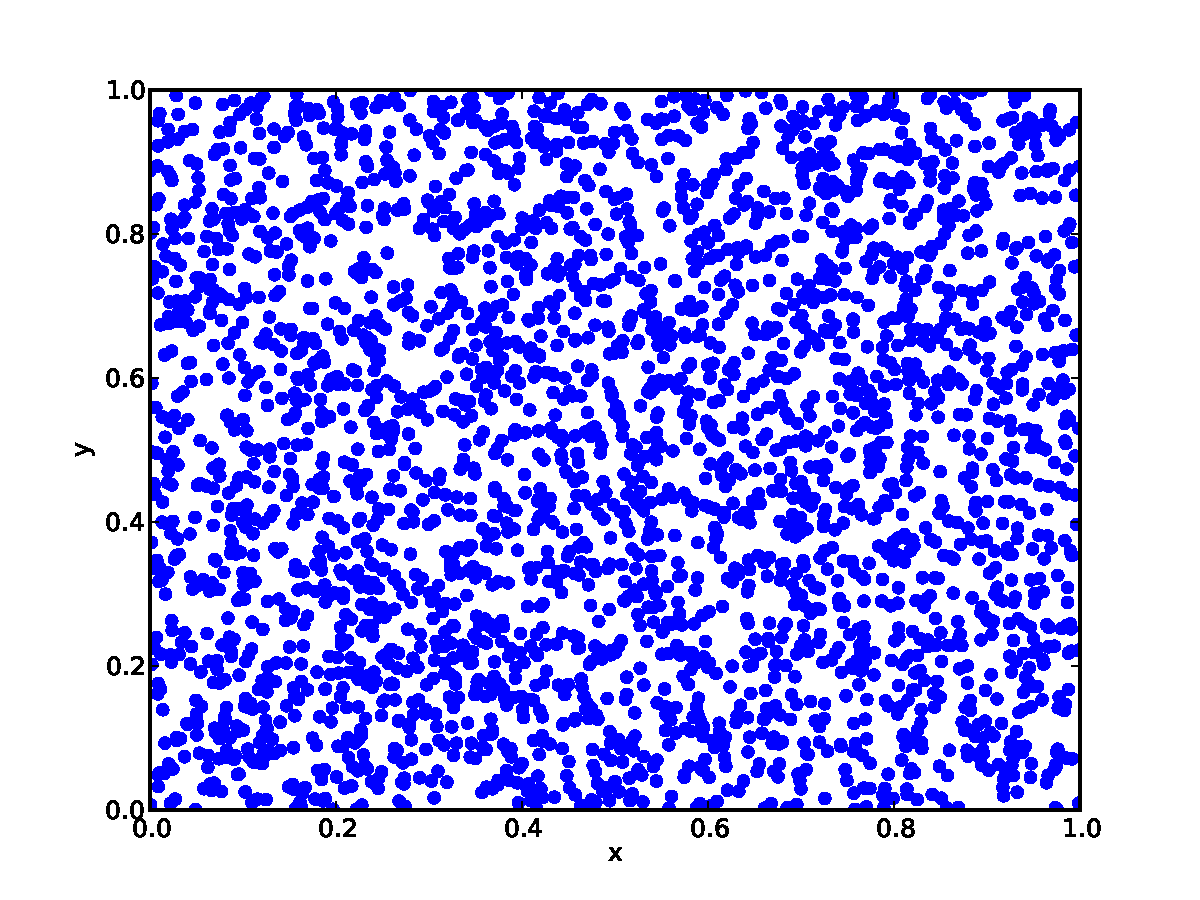
\includegraphics[scale=0.25]{figures/uniform_distribution.pdf}
		}
		\end{subfloat}~
	\end{center}

	\caption{Index Structure Performance With Respect To Dimensionality (10,000 Points from Uniform Distribution Synthetic Dataset)}
	\label{fig:perf3-dimensionality}
\end{figure}

\begin{table}
	\centering
	\makebox[\textwidth][c]{%
		\begin{tabular}{|r|r|l|l|l|l|}
			\hline
			\multicolumn{2}{|c}{} & \multicolumn{4}{|c|}{\textbf{Points in Dataset}} \\
			\hline
			\textbf{Structure} & \textbf{Operation} & 10,000 & 100,000 & 500,000 & 1,000,000 \\
			\hline
			\multirow{3}{*}{Bucket PPT} & Insert & TODO & TODO & TODO & TODO \\
				& Delete & TODO & TODO & TODO & TODO \\
				& PQuery & TODO & TODO & TODO & TODO \\
			\hline			
			\multirow{3}{*}{Bucket PT} & Insert & TODO & TODO & TODO & TODO \\
				& Delete & TODO & TODO & TODO & TODO \\
				& PQuery & TODO & TODO & TODO & TODO \\
			\hline			
			\multirow{3}{*}{Bucket Hash Table} & Insert & TODO & TODO & TODO & TODO \\
				& Delete & TODO & TODO & TODO & TODO \\
				& PQuery & TODO & TODO & TODO & TODO \\
			\hline
			\multirow{3}{*}{Point $kd$-Tree} & Insert & TODO & TODO & TODO & TODO \\
				& Delete & TODO & TODO & TODO & TODO \\
				& PQuery & TODO & TODO & TODO & TODO \\
			\hline
			\multirow{3}{*}{Bucket $kd$-Tree} & Insert & TODO & TODO & TODO & TODO \\
				& Delete & TODO & TODO & TODO & TODO \\
				& PQuery & TODO & TODO & TODO & TODO \\
			\hline
		\end{tabular}
	}%

	\caption{Total Execution Time (in seconds) of Each Operation for Varying Number of Points in Uniformly Distributed Synthetic Dataset}
	\label{tab:perf3-size}
\end{table}

\begin{figure}
	\begin{center}
		\begin{subfloat}[\texttt{insert}\label{fig:perf3-size-insert}]{%
			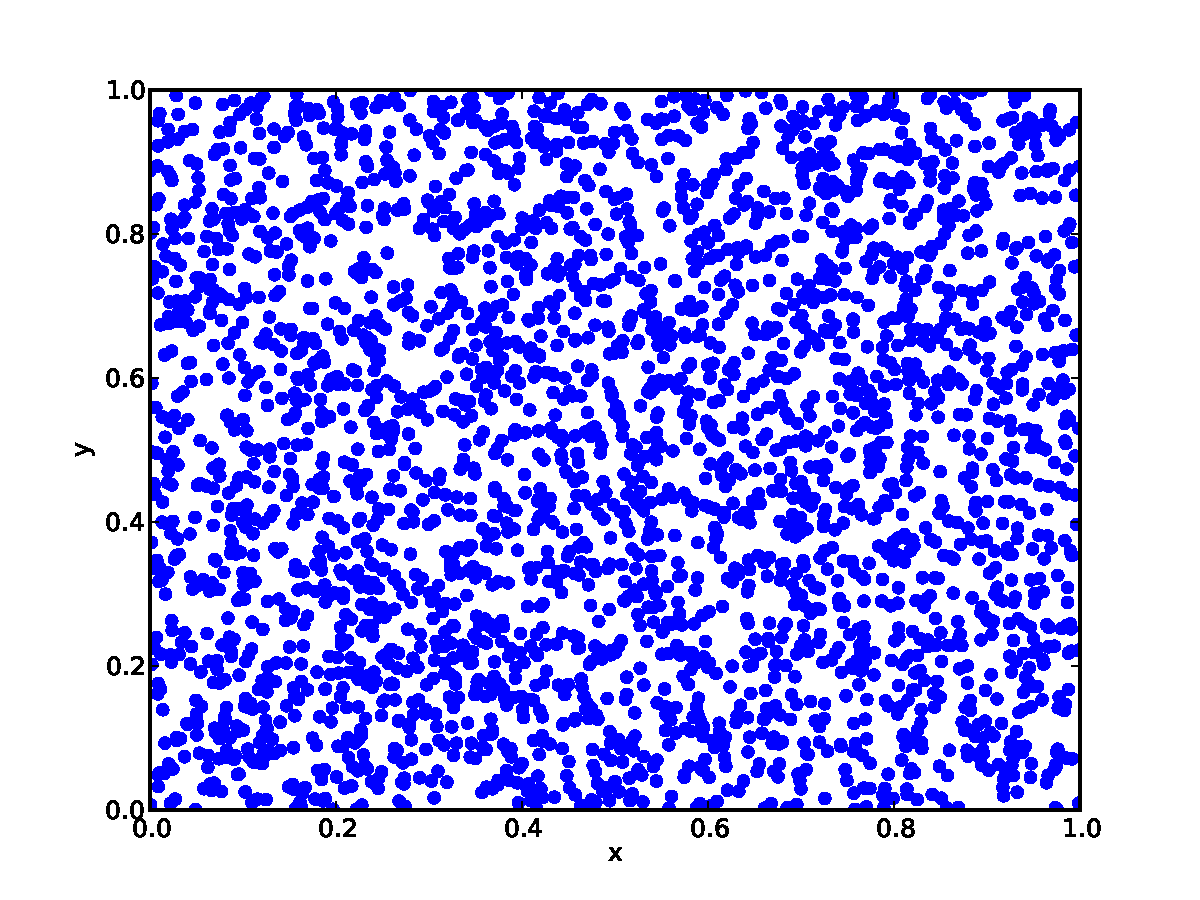
\includegraphics[scale=0.25]{figures/uniform_distribution.pdf}
		}
		\end{subfloat}~
		\begin{subfloat}[\texttt{remove}\label{fig:perf3-size-remove}]{%
			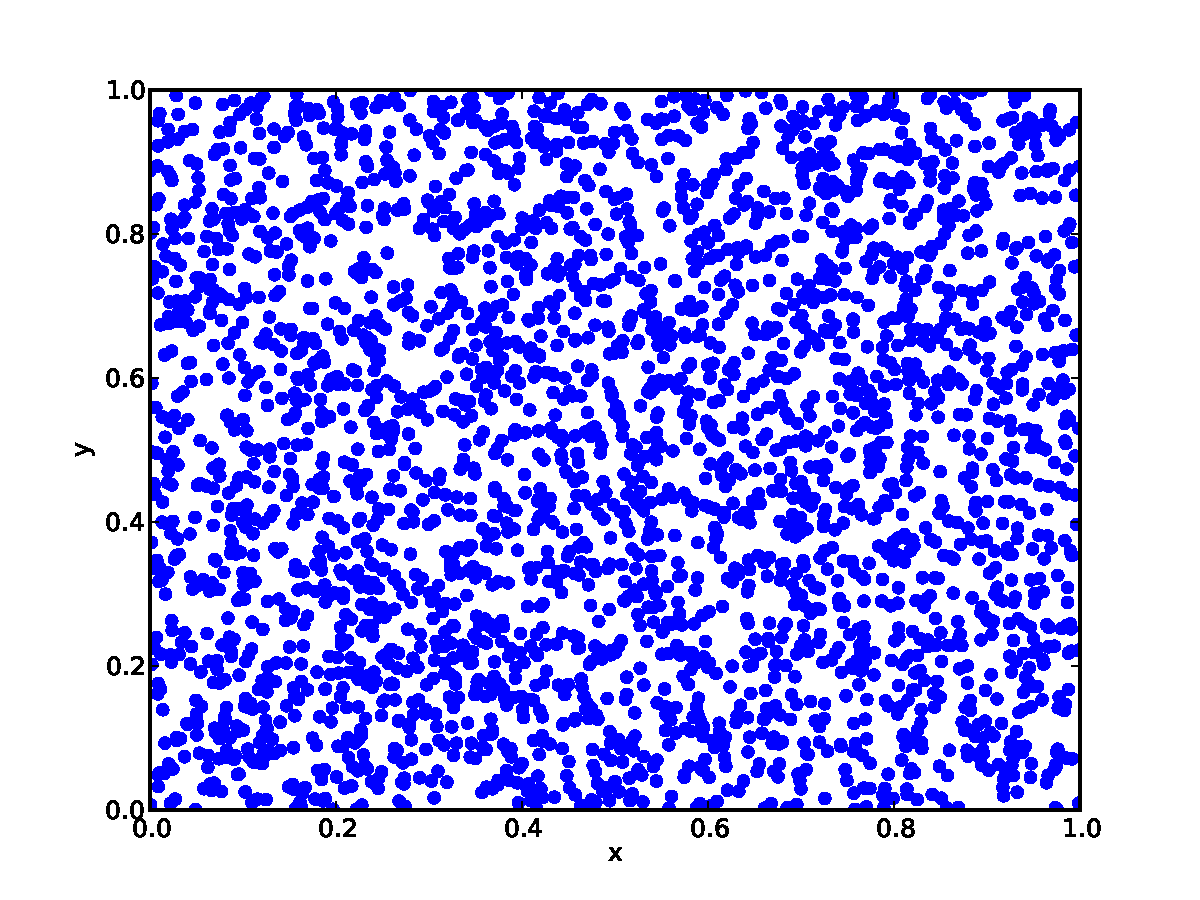
\includegraphics[scale=0.25]{figures/uniform_distribution.pdf}
		}
		\end{subfloat}~
	\end{center}

	\caption{Index Structure Performance With Respect To Dataset Size (10,000 Points from Uniform Distribution Synthetic Dataset)}
	\label{fig:perf3-size}
\end{figure}


\begin{table}
	\centering
	\makebox[\textwidth][c]{%
		\begin{tabular}{|r|r|l|l|l|}
			\hline
			\multicolumn{2}{|c}{} & \multicolumn{3}{|c|}{\textbf{Dataset}} \\
			\hline
			\textbf{Structure} & \textbf{Operation} & \textbf{Astrophysics} & \textbf{Hurricane Isabel} & \textbf{Armadillo Mesh} \\
			\hline
			\multirow{4}{*}{Bucket PPT} & Insert & TODO & TODO & TODO \\
				& Delete & TODO & TODO & TODO \\
				& PQuery & TODO & TODO & TODO \\
				& Random Operation List & TODO & TODO & TODO \\
			\hline
			\multirow{4}{*}{Bucket PT} & Insert & TODO & TODO & TODO \\
				& Delete & TODO & TODO & TODO \\
				& PQuery & TODO & TODO & TODO \\
				& Random Operation List & TODO & TODO & TODO \\
			\hline
			\multirow{4}{*}{Bucket Hash Table} & Insert & TODO & TODO & TODO \\
				& Delete & TODO & TODO & TODO \\
				& PQuery & TODO & TODO & TODO \\
				& Random Operation List & TODO & TODO & TODO \\
			\hline
			\multirow{4}{*}{Point $kd$-Tree} & Insert & TODO & TODO & TODO \\
				& Delete & TODO & TODO & TODO \\
				& PQuery & TODO & TODO & TODO \\
				& Random Operation List & TODO & TODO & TODO \\
			\hline
			\multirow{4}{*}{Bucket $kd$-Tree} & Insert & TODO & TODO & TODO \\
				& Delete & TODO & TODO & TODO \\
				& PQuery & TODO & TODO & TODO \\
				& Random Operation List & TODO & TODO & TODO \\
			\hline
		\end{tabular}
	}%

	\caption{Total Execution Time (in seconds) of Each Operation for 500,000 Points Sampled From Real Datasets}
	\label{tab:perf3-real}
\end{table}


\subsection{Profiling Results}

TODO

\begin{table}
	\centering
	\makebox[\textwidth][c]{%
		\begin{tabular}{|l|l|l|l|}
			\hline
			\textbf{Structure} & \textbf{Max Heap Memory (MB)} & \textbf{Cache Hit Rate (\%)} & \textbf{Dominant Function (\% Total Time Spent)} \\
			\hline
			Bucket PPT & TODO & TODO & TODO (TODO) \\
			Bucket PT & TODO & TODO & TODO (TODO) \\
			Bucket Hash Table & TODO & TODO & TODO (TODO) \\
			Point $kd$-Tree  & TODO & TODO & TODO (TODO) \\
			Bucket $kd$-Tree & TODO & TODO & TODO (TODO) \\
			\hline
		\end{tabular}
	}%
	\caption{CPU and Heap Profiling Statistics When Inserting 500,000 Points from 16D Synthetic Dataset into Index Structures}
	\label{tab:perf3-profiling}
\end{table}


\subsection{Summary}

TODO